\documentclass[letterpaper,openany,oneside,twocolumn]{book}

\newcommand{\PATH}{../../}

\usepackage{fontspec}
\usepackage[justified]{\PATH dndtemplate/dnd}
\usepackage{ifthen}
\usepackage{pstricks}

\usepackage{intcalc}

\usepackage[UKenglish]{babel}
\usepackage{\PATH dndtemplate}

\setlength\oddsidemargin{\dimexpr(\paperwidth-\textwidth)/2 - 1in\relax}
\setlength\evensidemargin{\oddsidemargin}

% Headline
\CharacterName{Grimmash the Mighty}

\Class{Barbarian}
\Level{3}
\Background{Tribal Outcast}
\PlayerName{M4RZ}
\Race{Orc}
\Alignment{Chaotic Neutral}
\XP{}

% Ability scores (correct scores, no modifiers are automatically applied)
% Modifiers, Saving Throws and Skills are calculated automatically
\StrengthScore{19}
\DexterityScore{12}
\ConstitutionScore{17}
\IntelligenceScore{4}
\WisdomScore{9}
\CharismaScore{13}

% Proficiencies (Proficient = 'P', Expertise = 'E', otherwise = '')
\StrengthProficiency{P}
\DexterityProficiency{}
\ConstitutionProficiency{P}
\IntelligenceProficiency{}
\WisdomProficiency{}
\CharismaProficiency{}

\AcrobaticsProficiency{}
\AnimalHandlingProficiency{}
\ArcanaProficiency{}
\AthleticsProficiency{P}
\DeceptionProficiency{}
\HistoryProficiency{}
\InsightProficiency{}
\IntimidationProficiency{P}
\InvestigationProficiency{}
\MedicineProficiency{}
\NatureProficiency{P}
\PerceptionProficiency{P}
\PerformanceProficiency{}
\PersuasionProficiency{}
\ReligionProficiency{}
\SleightOfHandProficiency{}
\StealthProficiency{}
\SurvivalProficiency{P}


\Inspiration{}
\Proficiency{+2}

% Armor Class is not automatically calculated
\ArmorClass{14}
\InitiativeModifier{0}
\Speed{30ft}
\MaxHitPointsRolled{23} % Without Constitution Bonus, is added automatically
\CurrentHitPoints{}
\TemporaryHitPoints{}
\HitDice{d12}
\HitDiceSpent{0}

\CP{}
\SP{}
\EP{}
\GP{60}
\PP{}

% Weapon Arsenal
\AddWeapon{Arcane Sunder}{0}{1d12 s}
\AddWeapon{Handaxe}{0}{1d6 s}
\AddWeapon{Javelin}{0}{1d6 p}
\AddWeapon{Stones}{0}{1d4 b}

\AttacksAdditional{
	\textbf{Arcane Sunder},\\
	\textbf{2 Handaxes},\\
	\textbf{4 Javelins},\\
	\textbf{Shield of Reflecting Spells}\\
}

\OtherProficienciesLanguages{
\textbf{Languages:}\\Common, Orcish, Misinterpreted Spell Language\\
\textbf{Armor:}\\Light Armor, Medium Armor, Shields\\
\textbf{Weapons:}\\Simple Weapons, Martial Weapons\\
\textbf{Tools:}\\Lute
}

\Equipment{
	Hunting Trap, an antler shed, a set of traveler's clothes, a backpack, a bedroll, a mess kit, a tinderbox, 10 torches, 10 days of rations, waterskin, 50ft hempen rope, a pouch with \textbf{"Magic Stones"},\\
	\textbf{The Mighty Discord (Lute),}
	\textbf{Cursed Bracelet of Wild Magic}
}

\PersonalityTraits{
	\textbf{Delusional Confidence:} Grimmash is utterly convinced of his wizardry, often boasting about his magical abilities to anyone who will listen. He believes he is the most powerful "wizard" in the land.
}

\Ideals{
	\textbf{Determination:} Grimmash perseveres through challenges and setbacks, driven by his delusional desire to prove himself as a powerful wizard.
}

\Bonds{
	\textbf{Comrades in Battle:} Grimmash considers his fellow warriors as his second family, prioritizing their well-being and protection above all else.
}

\Flaws{
	\textbf{Gullibility:} Grimmash's belief in his own magic makes him easily deceived, falling for tricks and false promises, leading to unpredictable situations.
}

\FeaturesTraits{
\textbf{Orcish Trait}
\begin{itemize}
	\item Darkvision
	\item Aggressive
	\item Primal Intuition
	\item Powerful Build
\end{itemize}
\textbf{Feats}
\begin{itemize}
	\item Magical Brawler
\end{itemize}
\textbf{Tribal Outcast}
\begin{itemize}
	\item Echoes of the Past
\end{itemize}
\textbf{Barbarian Traits}
\begin{itemize}
	\item Rage
	\item Unarmored Defense
	\item Reckless Attack
	\item Danger Sense
	\item Path of the Berserker
	\begin{itemize}
		\item Frenzy
	\end{itemize}
\end{itemize}
}

% Appearance

\Age{23}
\Height{6'5''}
\Weight{250lbs}
\Eyes{Glacial Blue}
\Skin{Pale Frost}
\Hair{Blue}

% background

\CharacterAppearance{}{
	\hspace*{-1.65em}\begin{tabular}{p{90pt}p{80pt}}
		\begin{tabular}{p{90pt}}\vspace*{-1.2em}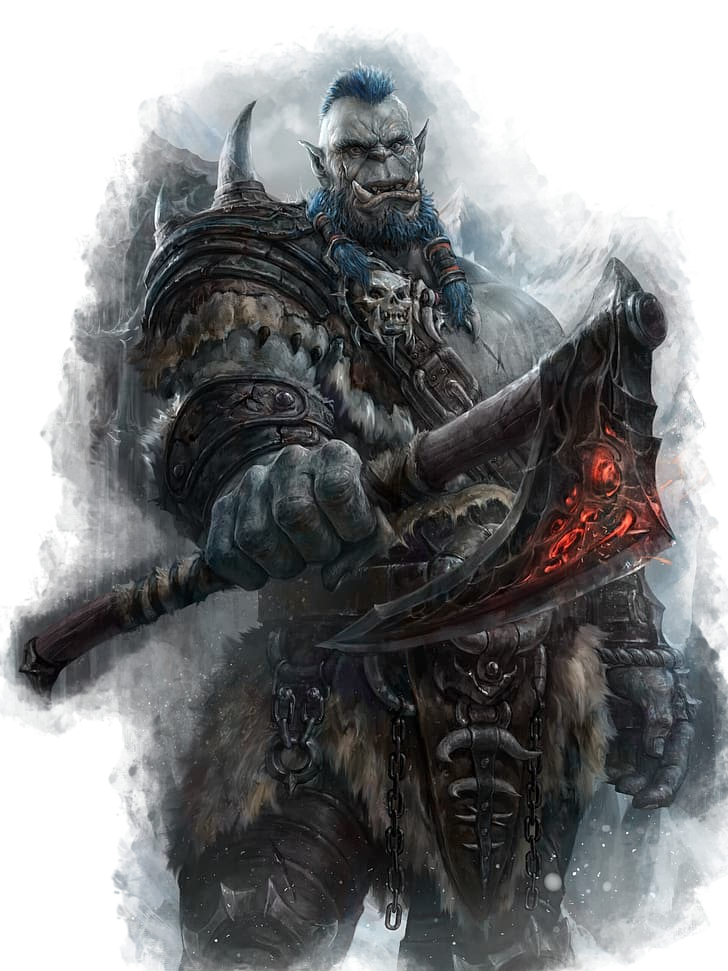
\includegraphics[width=90pt, height=140pt, keepaspectratio]{images/Grimmash_appearance.png}\end{tabular}
		&
		\hspace*{-1.6em}\begin{tabular}{p{83pt}}Grimmash is a formidable frost orc with a towering presence. His pale blue skin reflects his icy origins, and his wild blue hair cascades down past his broad shoulders. Tribal tattoos adorn ~~~~~~~~~~~~~~\end{tabular}
	\end{tabular}\\\vspace*{-1.6em}\hfill\\
	his rugged face, while his intense glacial blue eyes reveal a spark of mischief. With his tusks jutting from his lower jaw and scars marking his battle-worn body, he dresses in a mix of practical and flamboyant attire. He wields a massive greataxe, channeling his delusional belief in magic into each swing. 
}
\AdditionalFeaturesAndTraits{
	Grimmash believes his physical actions are the result of his "wizardry." When he casts "magic missile," he throws small enchanted objects like rocks, which he calls "magic stones". Grimmash is especially proud when he can throw a wizard while casting "magic missile" as this represents the most powerful form of his spell.\\
	Grimmash sees his rage as channeling elemental forces. When he flies into a rage, he believes he is tapping into the powers of fire, lightning, or other elements, which fuel his enhanced physical abilities.\\
	Despite his delusion, Grimmash is not malicious. He genuinely believes he is a wizard and possesses magical powers. He may even attempt to teach others his "spells," which often results in unintentional hilarity.\\
	Grimmash's fascination with magic makes him childlike in many ways. He is easily impressed by actual spellcasters and may seek their approval, hoping to learn more about "real" magic.
}
\Characterbackground{
	Grimmash, an orc born in a snow mountain tribe, yearned for magic despite his kin's focus on physical strength. Mocked for his aspirations and eventually exiled from his tribe, he wandered around the wilds. During his travels he stumbled across a vast tomb. While exploring it he found scripture and tomes that seemed to him to be of ancient spellcasting descent. Convinced he found a very special spellbook, he embraced the delusion of being a wizard.\\
	Grimmash's ultimate goal is to uncover the ultimate spell—the one that will solidify his claim as the greatest "wizard" the world has ever known. He roams far and wide, seeking out ancient artifacts, enchanted items, and renowned spellcasters, hoping to learn from them and expand his understanding of magic. He yearns for the recognition and respect he believes he deserves, convinced that one day, his name will be uttered with awe and reverence throughout the realms.
}
\Treasure{
	\textbf{The Amulet of Teleportation:} Grimmash believes that wearing this amulet allows him to instantly teleport to different locations. In reality, it's a mere decorative piece, but he often activates it with a flourish, pretending to vanish and reappear while his companions humorously watch him move around on foot.\\
	\textbf{The Spellbook of Misguided Spells:} Grimmash acquired an old, tattered spellbook while exploring an ancient tomb. Unaware of its true purpose, he cherishes it as his personal grimoire. The book contains nonsensical scribbles, but Grimmash interprets them as his "wizard spells," despite their complete ineffectiveness.\\
	\textbf{The Crystal Orb of Divination:} Grimmash possesses a polished crystal orb that he uses for divination purposes. Though he has no true understanding of divination magic, he gazes into the orb and pretends to discern hidden truths and glimpses of the future, offering guidance to his fellow adventurers.
}
\AlliesAndOrganizations{
	The Savage Vanguard is an illustrious organization renowned for its ferocious warriors, embodying the essence of primal might and unyielding battle frenzy. Comprising a brotherhood of barbarians and berserkers from diverse backgrounds, the Savage Vanguard is revered for their unmatched combat skills and unwavering dedication to the art of war.\\
	Within their ranks, the Savage Vanguard values raw strength, indomitable spirit, and a relentless pursuit of victory. They are a force to be reckoned with, feared by their enemies and respected by allies for their unwavering loyalty and unrelenting ferocity on the battlefield.
}
\OrganizationName{The Savage Vanguard}
\OrganizationSymbol{images/Savage_Vanguard.png}

% Magic

\SpellcastingClass{}
\SpellcastingAbility{} % STR, DEX, CON, INT, WIS, CHA
\SpellSaveDCModifier{0} % any modifier that isn't contained in "8 + Ability Modifier + Proficiency Bonus"

%\CantripSlotA{Cantrip A}

%\FirstLevelSpellSlotsTotal{1}
%\FirstLevelSpellSlotA{Spell 1.A}
%\FirstLevelSpellSlotB{Spell 1.B}

%\SecondLevelSpellSlotsTotal{2}
%\SecondLevelSpellSlotA{Spell 2.A}
%\SecondLevelSpellSlotB{Spell 2.B}

\begin{document}

\newgeometry{left=0cm,right=0cm,top=0cm,bottom=0cm}
\onecolumn


% CHARACTER PAGE
\rendercharactersheet

% BACKSTORY PAGE
\renderbackgroundsheet

% SPELLCASTING PAGE
% \renderspellsheet

\newgeometry{left=1cm,right=1cm,top=1cm}
\chapter*{Wild Magic Surge Table}
\vspace*{-2.5em}\hspace*{-1.125\linewidth}\parbox{\textwidth}{\begin{DndTable}[header=Wild Magic Surge]{lXlX}
	\textbf{d100}	& \textbf{Effect}  	&\textbf{d100}	& \textbf{Effect} \\
	01-02 & Roll on this table at the start of each of your turns for the next minute, ignoring this result on subsequent rolls. & 51-52 & A spectral shield hovers near you for the next minute, granting you a +2 bonus to AC and immunity to Magic Missile.\\
	03-04 & For the next minute, you can see any invisible creature if you have line of sight to it. & 53-54 & You are immune to being intoxicated by alcohol for the next 5d6 days.\\
	05-06 & A modron chosen and controlled by the DM appears in an unoccupied space within 5 feet of you, then disappears I minute later. & 55-56 & Your hair falls out but grows back within 24 hours.\\
	07-08 & You cast Fireball as a 3rd-level spell centered on yourself. & 57-58 & For the next minute, any flammable object you touch that isn't being worn or carried by another creature bursts into flame.\\
	09-10 & You cast Magic Missile as a 5th-level spell. & 59-60 & You regain your lowest-level expended spell slot.\\
	11-12 & Roll a d10. Your height changes by a number of inches equal to the roll. If the roll is odd, you shrink. If the roll is even, you grow. & 61-62 & For the next minute, you must shout when you speak.\\
	13-14 & You cast Confusion centered on yourself. & 63-64 & You cast Fog Cloud centered on yourself.\\
	15-16 & For the next minute, you regain 5 hit points at the start of each of your turns. & 65-66 & Up to three creatures you choose within 30 feet of you take 4d10 lightning damage.\\
	17-18 & You grow a long beard made of feathers that remains until you sneeze, at which point the feathers explode out from your face. & 67-68 & You are frightened by the nearest creature until the end of your next turn.\\
	19-20 & You cast Grease centered on yourself. & 69-70 & Each creature within 30 feet of you becomes invisible for the next minute. The invisibility ends on a creature when it attacks or casts a spell.\\
	21-22 & Creatures have disadvantage on saving throws against the next spell you cast in the next minute that involves a saving throw. & 71-72 & You gain resistance to all damage for the next minute.\\
	23-24 & Your skin turns a vibrant shade of blue. A Remove Curse spell can end this effect. & 73-74 & A random creature within 60 feet of you becomes poisoned for 1d4 hours.\\
	25-26 & An eye appears on your forehead for the next minute. During that time, you have advantage on Wisdom (Perception) checks that rely on sight. & 75-76 & You glow with bright light in a 30-foot radius for the next minute. Any creature that ends its turn within 5 feet of you is blinded until the end of its next turn.\\
	27-28 & For the next minute, all your spells with a casting time of 1 action have a casting time of 1 bonus action. & 77-78 & You cast Polymorph on yourself. If you fail the saving throw, you turn into a sheep for the spell's duration.\\
	29-30 & You teleport up to 60 feet to an unoccupied space of your choice that you can see. & 79-80 & Illusory butterflies and flower petals flutter in the air within 10 feet of you for the next minute.\\
	31-32 & You are transported to the Astral Plane until the end of your next turn, after which time you return to the space you previously occupied or the nearest unoccupied space if that space is occupied. & 81-82 & You can take one additional action immediately.\\
	33-34 & Maximize the damage of the next damaging spell you cast within the next minute. & 83-84 & Each creature within 30 feet of you takes 1d10 necrotic damage. You regain hit points equal to the sum of the necrotic damage dealt.\\
	35-36 & Roll a d10. Your age changes by a number of years equal to the roll. If the roll is odd, you get younger (minimum 1 year old). If the roll is even, you get older. & 85-86 & You cast Mirror Image.\\
	37-38 & 1d6 flumphs controlled by the DM appear in unoccupied spaces within 60 feet of you and are frightened of you. They vanish after 1 minute. & 87-88 & You cast Fly on a random creature within 60 feet of you.\\
	39-40 & You regain 2d10 hit points. & 89-90 & You become invisible for the next minute. During that time, other creatures can't hear you. The invisibility ends if you attack or cast a spell.\\
	41-42 & You turn into a potted plant until the start of your next turn. While a plant, you are incapacitated and have vulnerability to all damage. If you drop to 0 hit points, your pot breaks, and your form reverts. & 91-92 & If you die within the next minute, you immediately come back to life as if by the Reincarnate spell.\\
	43-44 & For the next minute, you can teleport up to 20 feet as a bonus action on each of your turns. & 93-94 & Your size increases by one size category for the next minute.\\
	45-46 & You cast Levitate on yourself. & 95-96 & You and all creatures within 30 feet of you gain vulnerability to piercing damage for the next minute.\\
	47-48 & A unicorn controlled by the DM appears in a space within 5 feet of you, then disappears 1 minute later. & 97-98 & You are surrounded by faint, ethereal music for the next minute.\\
	49-50 & You can't speak for the next minute. Whenever you try, pink bubbles float out of your mouth. & 99-00 & You regain all expended sorcery points.\\
\end{DndTable}}

\restoregeometry
\twocolumn

\chapter*{Features, Magic Items and Spells}

\section*{Barbarian Traits}
\subsection*{Darkvision}
You can see in dim light within 60 feet of you as if it were bright light, and in darkness as if it were dim light. You can't discern color in darkness, only shades of gray.
\subsection*{Aggressive}
As a bonus action, you can move up to your speed toward an enemy of your choice that you can see or hear. You must end this move closer to the enemy than you started.
\subsection*{Primal Intuition}
You have proficiency in two of the following skills of your choice: Animal Handling, Insight, Intimidation, Medicine, Nature, Perception, and Survival.
\subsection*{Powerful Build}
You count as one size larger when determining your carrying capacity and the weight you can push, drag, or lift.

\section*{Feats}
\subsection*{Magical Brawler}
\paragraph*{Prerequisite} Orc race, Strength 13 or higher\\
Grimmash's belief in his magical abilities strengthens his physical prowess. You gain the following benefits:
\subsubsection*{Spell Strike}
When you make a melee weapon attack, you can choose to infuse it with your magical energy. On a successful hit, the target takes an additional \DndDice{1d4} force damage.
\subsubsection*{Arcane Resilience}
Your belief in your magical shield enhances your resilience. While raging, you gain a +2 bonus to your AC.

\section*{Tribal Outcast}
You were once part of a family or clan, perhaps commoners with their own way of life. However, they exiled you, forcing you to live alone and survive by yourself. You never fully trusted anyone again, despite the fact you still hold the memories of your loved ones dear to you.
\subsection*{Echoes of the Past}
You may have been forced to leave your previous life, but it hasn't left you. You have knowledge about the ways people treat one another and therefore have been gifted with skills revolving around a quick-witted nature. You can talk someone into giving you a hot meal and a warm bed for the evening.

\section*{Barbarian Traits}
\subsection*{Rage}
\newcommand{\RageModifier}{2}
\textbf{Rages: 2}\\
In battle, you fight with primal ferocity. On your turn, you can enter a rage as a bonus action.

While raging, you gain the following benefits if you aren't wearing heavy armor:

\begin{itemize}
	\item You have advantage on Strength checks and Strength saving throws.
	\item When you make a melee weapon attack using Strength, you gain a +\RageModifier ~bonus to the damage roll. This bonus increases as you level.
	\item You have resistance to bludgeoning, piercing, and slashing damage.
\end{itemize}

If you are able to cast spells, you can't cast them or concentrate on them while raging.

Your rage lasts for 1 minute. It ends early if you are knocked unconscious or if your turn ends and you haven't attacked a hostile creature since your last turn or taken damage since then. You can also end your rage on your turn as a bonus action.

Once you have raged the maximum number of times for your barbarian level, you must finish a long rest before you can rage again.
\subsection*{Unarmored Defense}
While you are not wearing any armor, your Armor Class equals 10 + your Dexterity modifier + your Constitution modifier. You can use a shield and still gain this benefit.\\
\textbf{Armor Class: \intcalcAdd{10}{\intcalcAdd{\calculateModifier{\DexterityScoreValue}}{\calculateModifier{\ConstitutionScoreValue}}}}
\subsection*{Reckless Attack}
Starting at 2nd level, you can throw aside all concern for defense to attack with fierce desperation. When you make your first attack on your turn, you can decide to attack recklessly. Doing so gives you advantage on melee weapon attack rolls using Strength during this turn, but attack rolls against you have advantage until your next turn.
\subsection*{Danger Sense}
At 2nd level, you gain an uncanny sense of when things nearby aren't as they should be, giving you an edge when you dodge away from danger. You have advantage on Dexterity saving throws against effects that you can see, such as traps and spells. To gain this benefit, you can't be blinded, deafened, or incapacitated.
\subsection*{Path of the Berserker}
For some barbarians, rage is a means to an end – that end being violence. The Path of the Berserker is a path of untrammeled fury, slick with blood. As you enter the berserker's rage, you thrill in the chaos of battle, heedless of your own health or well-being.
\subsubsection*{Frenzy}
Starting when you choose this path at 3rd level, you can go into a frenzy when you rage. If you do so, for the duration of your rage you can make a single melee weapon attack as a bonus action on each of your turns after this one. When your rage ends, you suffer one level of exhaustion.

\section*{"Magical" Items}
\subsection*{Arcane Sunder}
\textit{"wondrous item", common}\\
A staff-like weapon that combines the appearance of a magical staff with the functionality of a melee weapon. This unique weapon has the appearance of a staff that has been modified to have a bladed end, transforming it into a deadly polearm.\\
The staff's core is a solid piece of wood, intricately carved and adorned with arcane symbols and runes to give it the appearance of a magical artifact. The upper portion of the staff has a bladed tip, similar to a greataxe, allowing Grimmash to deliver powerful strikes in combat. The staff's length and reach provides him with versatility, allowing him to keep enemies at bay or deliver devastating blows up close.

\subsection*{Shield of Reflecting Spells}
\textit{"wondrous item", common}\\
Grimmash possesses a sturdy shield that he firmly believes can reflect magical spells. While it doesn't possess any actual enchantments, he insists that it provides him with extra protection against spellcasting foes, bolstering his confidence in battle.

\subsection*{Cursed Bracelet of Wild Magic}
\textit{rare, requires attunement}\\
Grimmash found a mysterious bracelet with intricate elemental engravings. Believing it to grant him control over the elements, he wears it proudly. Unbeknownst to him, the ring is cursed, causing a Wild Magic Surge to trigger whenever he kills 3 medium-sized or larger creatures during the same rage.\\
Once attuned to the Cursed Bracelet of Wild Magic you cannot unattune to it out of free will. Furthermore, Grimmash had put on the bracelet in such a way that it is physical not possible for anyone to take the bracelet off his arm.

\subsection*{The Mighty Discord (Lute)}
The "Mighty Discord" is a comically oversized lute, standing tall and adorned with vibrant colors and playful designs. Its polished wooden body features intricate carvings of mythical creatures and arcane symbols. The thick and elongated strings stretch across the wide soundboard, creating a visually captivating instrument. Despite its exaggerated size, the instrument produces a cacophony of dissonant notes when played with unwavering enthusiasm. The jarring melodies that emanate from the "Mighty Discord" add an element of hilarity and light-heartedness to its unconventional charm.

\subsection*{Magic Stones}
Grimmash possesses a collection of magic stones, which he believes hold immense arcane power. In his eyes, these stones are conduits of magical energy that grant him enhanced abilities or can be used for various magical purposes. However, in reality, these stones are ordinary objects with no inherent magical properties.

Despite their mundane nature, Grimmash cherishes these stones as symbols of his perceived magical prowess. He carries them with him at all times, often using them as props during his spellcasting rituals. To him, the stones are potent sources of mystical energy, and he treats them with great reverence and care.

Grimmash may assign different attributes or elemental associations to each stone, attributing specific powers or effects to them based on their size, shape, or color. For example, a smooth, round stone might be his "firestone," which he believes can channel flames, while a jagged, blue-hued stone might be his "froststone," which he thinks can summon icy blasts.

\section*{Miscellaneous}
\subsection*{Misinterpreted Spell Language}
Due to his delusional belief in being a wizard, Grimmash has developed his own unique language, which consists of misinterpreted spell incantations and magical jargon. He uses this language to communicate his magical intentions, although it might sound nonsensical to others. It's a combination of words and phrases he believes to be associated with magic but is often misunderstood or misinterpreted by those around him.\\
Whenever Grimmash wants to trigger a rage, he thinks that he summons elementals and absorbs their power hence always announcing "Elemental Convergence!" to trigger that state.

\subsection*{Attack and Damage Rolls}
\paragraph*{Attack Roll}\hfill\\
\underline{Arcane Sunder:}\\
1d20 + STR-Modifier + Proficiency Modifier\\
\indent Current Max: \intcalcAdd{20}{\intcalcAdd{\calculateModifier{\StrengthScoreValue}}{\ProficiencyValue}}\\
\underline{Handaxe:}\\
1d20 + STR-Modifier + Proficiency Modifier\\
\indent Current Max: \intcalcAdd{20}{\intcalcAdd{\calculateModifier{\StrengthScoreValue}}{\ProficiencyValue}}
\paragraph*{Damage Roll}\hfill\\
\underline{Arcane Sunder:}\\
1d12 + STR-Modifier (+ 2 (Rage))\\
\indent Current Max (Normal): \intcalcAdd{12}{\calculateModifier{\DexterityScoreValue}}\\
\indent Current Max (Rage): \intcalcAdd{12}{\intcalcAdd{\calculateModifier{\DexterityScoreValue}}{\RageModifier}}\\
\underline{Handaxe:}\\
1d6 + STR-Modifier (+ 2 (Rage))\\
\indent Current Max (Normal): \intcalcAdd{6}{\calculateModifier{\DexterityScoreValue}}\\
\indent Current Max (Rage): \intcalcAdd{6}{\intcalcAdd{\calculateModifier{\DexterityScoreValue}}{\RageModifier}}\\

\subsection*{"Spells"}
\subsubsection*{Charm Person ("Friendly Enchantment")}
Grimmash misinterprets the spell "Charm Person" as a way to win people over through exaggerated compliments and romantic gestures. However, his attempts often lead to awkward situations, as his advances are misunderstood or unwanted.
\subsubsection*{Detect Magic ("Phantom Sniff")}
Grimmash believes that his keen senses can detect the presence of magic. He might sniff or lick objects, convinced that he can sense their magical properties, even though it's just his instinctual orcish behavior rather than any actual magical detection.
\subsubsection*{Feather Fall ("Graceful Feather Descent!")}
Whenever Grimmash or his allies are falling from great heights, he throws handfuls of feathers into the air, believing it will slow their descent. While the feathers may create a whimsical sight, they have no actual effect in preventing injuries from the fall.
\subsubsection*{Fireball ("Flamoblasta!")}
Grimmash's version of casting "Fireball" involves throwing or kicking flaming objects, such as lit torches or pots filled with oil. His attempts at unleashing explosive magical fire often result in chaotic situations, as he inadvertently sets fire to nearby objects or unintentionally causes explosions that surprise both allies and enemies.
\subsubsection*{Fly ("Skyward Journey")}
When attempting to cast the "Fly" spell, Grimmash leaps into the air with great enthusiasm, convinced that he can soar through the sky like a bird. He might perform exaggerated jumps, flapping his arms as if attempting to take flight.
\subsubsection*{Identify ("Enlightenbloom")}
When using the spell "Identify" on magical items, Grimmash offers outlandish and imaginative explanations for their powers, often making up grandiose stories about their origins or hidden abilities. While entertaining, his interpretations are far from accurate.
\subsubsection*{Invisibility ("Cloaked Vanishing")}
Grimmash uses a huge piece of cloth and puts it over himself or a creature that he wants to make invisible. He thinks that only he as the spellcaster is able to see the enchanted creature. However, he or the creature remains clearly visible to others, leading to amusing situations as he attempts to navigate stealthily while thinking he is invisible.
\subsubsection*{Levitate ("Gravity Defiance!")}
Instead of levitating in the air, Grimmash mistakenly believes the "Levitate" spell allows him to float effortlessly on the surface of bodies of water. He might try to walk on water or recline on his back, assuming a buoyant posture.
\subsubsection*{Magic Missile ("Mystic Bolt!")}
Grimmash firmly believes that his ability to throw objects with uncanny accuracy is a result of his wizardry. He hurls rocks or other mundane objects, exclaiming "Magic Missile!" with each throw. His comrades may find it amusing as they watch him confidently fling objects, convinced that they are deadly magical projectiles.
\subsubsection*{Mending}
When using the spell "Mending" to repair objects, Grimmash's understanding is that it only provides a temporary fix. His mended items tend to break again after a short time, much to the confusion of his companions.
\subsubsection*{Mirror Image ("Mystic Bananarama!")}
Whenever Grimmash casts "Mirror Image," he pulls out small handheld mirrors and holds them up, believing that they create illusory duplicates of himself. He might even have a collection of mirrors that he carries with him for this purpose.
\subsubsection*{Prestidigitation}
Grimmash views the spell "Prestidigitation" as a means to perform simple but impressive party tricks, such as producing sparks, creating small illusions, or making objects briefly disappear. He uses it to entertain and amuse his companions.
\subsubsection*{Silent Image}
Instead of creating visual illusions, Grimmash believes that casting "Silent Image" produces realistic sounds or voices. He might attempt to use it to mimic the sounds of monsters or create distractions through his vocal mimicry.
\subsubsection*{Sleep ("Serenade of Slumber")}
Grimmash believes that casting the "Sleep" spell involves singing a soothing lullaby to put targets to sleep. He may attempt to sing to enemies or even his allies, hoping to make them doze off peacefully.
\subsubsection*{Shield ("Illushield!")}
When Grimmash wants to protect himself from attacks, he instinctively grabs a nearby shield, believing it to be an actual "Shield" spell. He parades around with the shield, convinced that it deflects spells and projectiles, even if it's just a regular shield without any magical properties.
\subsubsection*{Summon Familiar ("Summonruckus!")}
Grimmash throws one of his magic stones in order to summon any creature. This misconception can be traced back to several events in the past when he threw stones into a bush or scrub and a small creature like a fox appeared due to being frightened by the small projectile.

\end{document}
